\documentclass{thesis-ekf}
\usepackage[T1]{fontenc}
\PassOptionsToPackage{defaults=hu-min}{magyar.ldf}
\usepackage[magyar]{babel}
\usepackage{mathtools,amssymb,amsthm,pdfpages}
\footnotestyle{rule=fourth}

\newtheorem{tetel}{Tétel}[chapter]
\theoremstyle{definition}
\newtheorem{definicio}[tetel]{Definíció}
\theoremstyle{remark}
\newtheorem{megjegyzes}[tetel]{Megjegyzés}

\usepackage{listings}
\usepackage{array}
\setlength{\extrarowheight}{2pt}

\begin{document}

\institute{Matematikai és Informatikai Intézet}
\title{\LaTeX beadandó}
\author{Zana Domán\\Programtervező informatikus}
\supervisor{Hekk Elek\\Tanársegéd}
\city{Eger}
\date{2025}
\maketitle

\tableofcontents

\chapter{Extra feladatok}

\section{Programkód}
\lstinputlisting[numbers=left,language=C,label={lst:reverse}]{reverse.c}
\Aref{lst:reverse} programkód rekurzió segítségével fordít meg egy karakterláncot.

\section{Táblázat}
\begin{table}[h]
    \centering
    \footnotesize
    \begin{tabular}{|>{\bfseries}l|l|l|l|l|l|}
        \cline{2-6}
        \multicolumn{1}{c|}{} & \multicolumn{5}{c|}{\textbf{Órarend}}\\
        \cline{2-6}
        \multicolumn{1}{c|}{} &
        \multicolumn{1}{c|}{\textbf{Hétfő}} &
        \multicolumn{1}{c|}{\textbf{Kedd}} &
        \multicolumn{1}{c|}{\textbf{Szerda}} &
        \multicolumn{1}{c|}{\textbf{Csütörtök}} &
        \multicolumn{1}{c|}{\textbf{Péntek}} \\
        \hline
        08.00--08.45 & matematika & rajz & irodalom & angol & matematika\\
        \hline
        08.55--09.40 & ének-zene & testnevelés & matematika & kémia & történelem\\
        \hline
        09.50--10.35 & irodalom & matematika & angol & matematika & testnevelés\\
        \hline
        10.45--11.30 & nyelvtan & történelem & biológia & nyelvtan & angol\\
        \hline
    \end{tabular}
\end{table}

\begin{thebibliography}{2}
\addcontentsline{toc}{chapter}{\bibname}
\end{thebibliography}

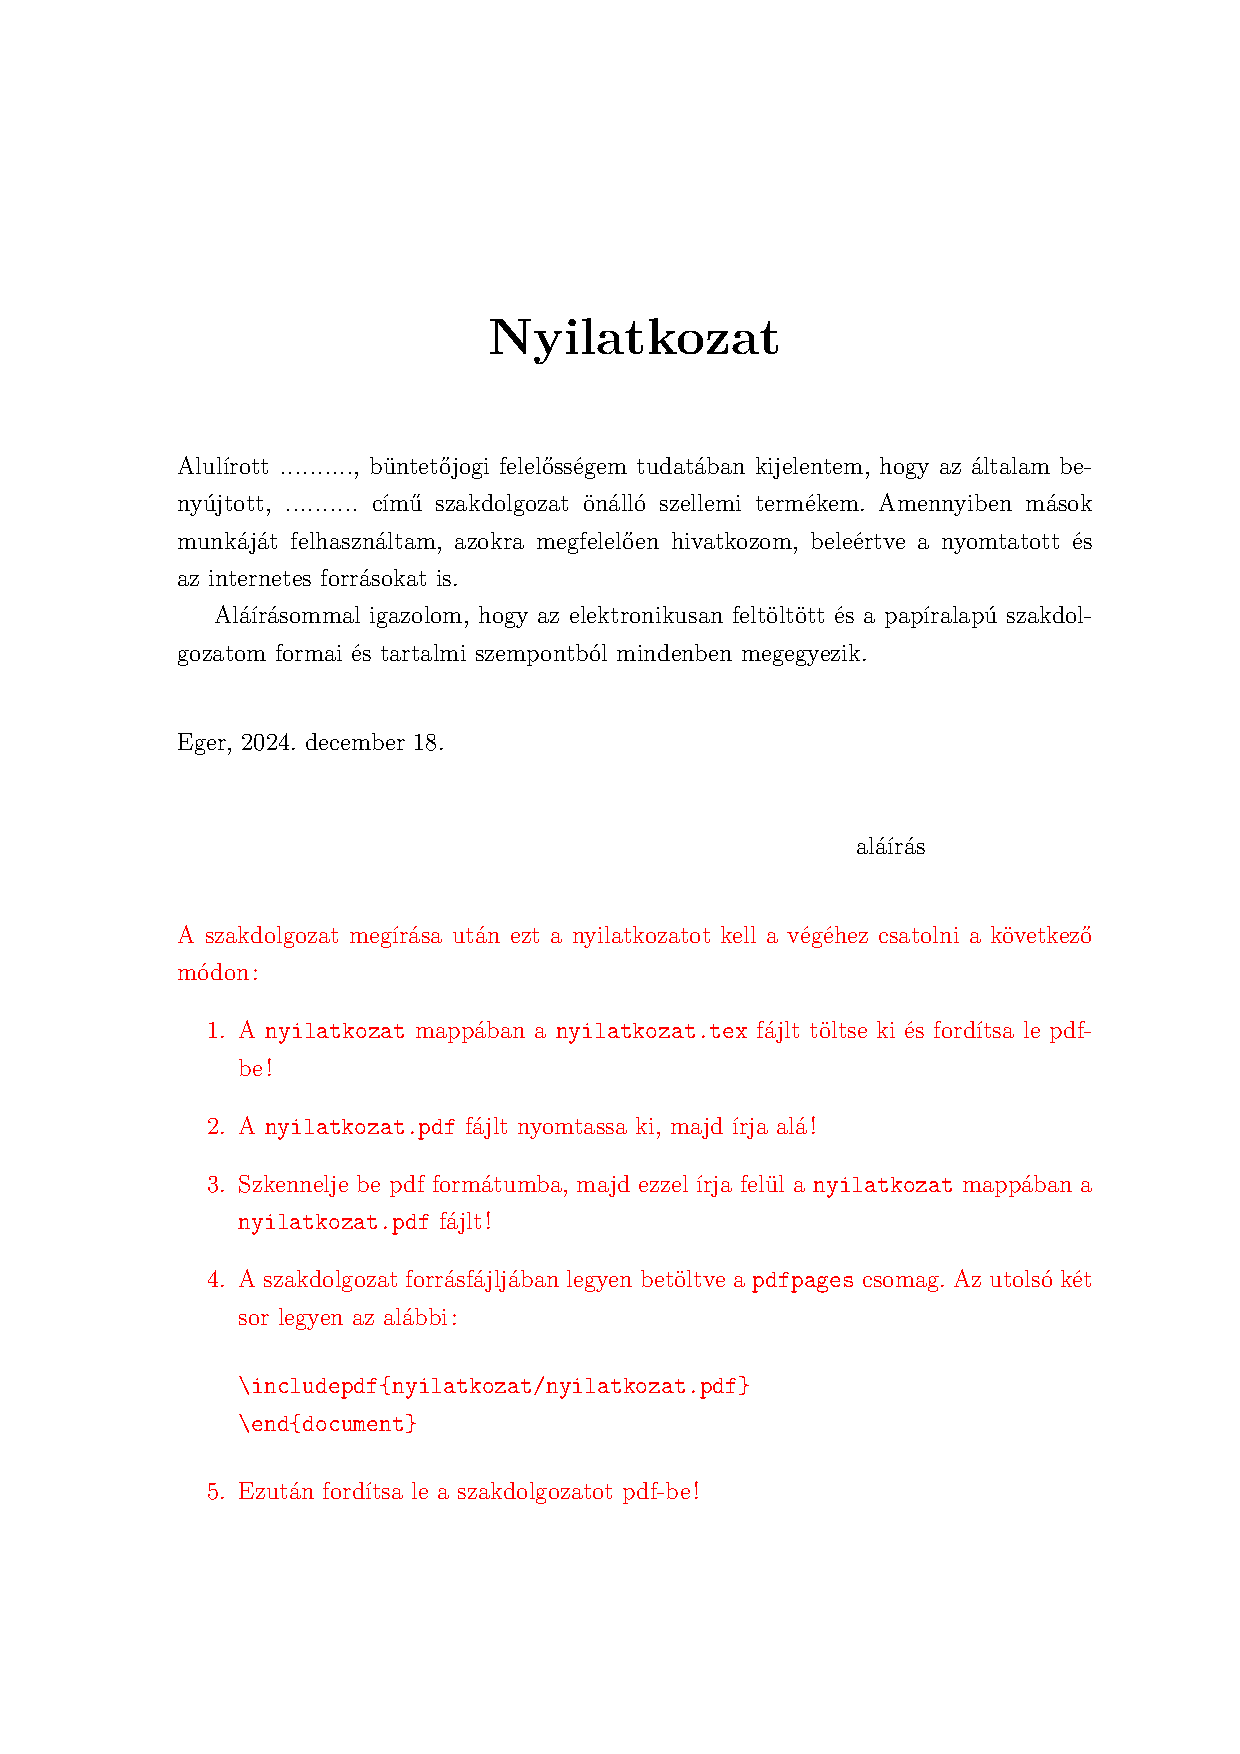
\includepdf{nyilatkozat/nyilatkozat.pdf}
\end{document}
